Vor dem Lebensende des Adobe Flash-Players im Dezember 2020 wurde dieser häufig zur Entwicklung von Browserbasierten Mehrspieler-Spielen verwendet. Diese Spiele wurden auf verschiedenen Plattformen wie zum Beispiel \textit{Newgrounds.com} angeboten. Der Flash-Player verfügte dabei über Peer-To-Peer-Fähigkeiten via Adobes \acf{RTMFP}. Somit bot der Flash-Player als Plattform eine kostengünstige Alternative zu Client-Server-Netzwerkarchitekturen. Mit dem Wegfall des Flash-Players ist WebRTC nun die einzige Technologie, welche ohne zusätzliche Software oder Plugins zum direkten Vernetzen von Browsern genutzt werden kann.\par

\acs{WebRTC} wird bereits in einigen Browserbasierten Mehrspieler-Spielen, sowie Networking- und Spiel-Frameworks verwendet. In der Regel wird WebRTC dabei jedoch lediglich für Sprach- und Videokommunikation eingesetzt. Die Strategie- und Brettspiel Plattform \textit{Jocly} ist eine der ersten Plattformen, welche bereits seit 2013 \acs{WebRTC} nutzt, damit Spieler sich in Echtzeit über ihre Webcams beim Spielen sehen, sowie miteinander kommunizieren können (vgl. Abbildung~\ref{fig:jocly}) \cite{jocly2013}. Ähnlich verhält es sich bei einigen weiteren Frameworks, wie zum Beispiel \textit{Tabloro}\footnote{vgl. \url{https://github.com/fyyyyy/tabloro}}, einem Browserbasierten \glqq{}Tabletop\grqq{}-Spielsimulator. Diese Spiele und Frameworks nutzen eine Client-Server-Architektur für den regulären (nicht Video und Audio) Datenaustausch.\par

\begin{figure}[h]
\centering
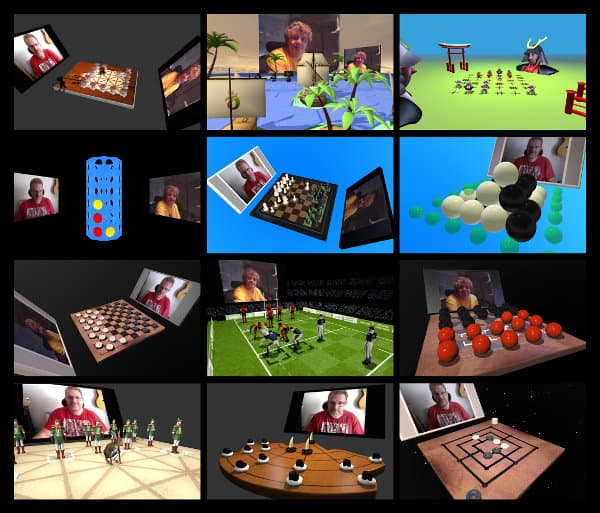
\includegraphics[width=0.70\textwidth]{bilder/jocly-games.jpg}
\caption{Einige Jocly-Spiele, mit WebRTC Videokommunikation.}
\source{\url{https://bloggeek.me/jocly-webrtc-interview/}}
\label{fig:jocly}
\end{figure}

Weiterhin existieren eine Reihe an prototypischen Spielen und Frameworks, welche \acs{WebRTC} zum Austausch von Daten nutzen. Bei diesen handelt es sich überwiegend um Echtzeitspiele wie das 2013 von Google entwickelte \textit{CubeSlam}. Abbildung~\ref{fig:cuubslam} zeigt dabei eine Bildschirmaufname eines CubeSlam-Spiels. CubeSlam nutzt \acs{WebRTC} Medienstreams, um Videodaten zu übertragen, und Datenkanäle, um die Spieldaten zwischen den Spielern zu synchronisieren. Auch der 2012 von Mozilla entwickelte First-Person-Shooter \textit{Bananabread}\footnote{vgl. \url{https://hacks.mozilla.org/2013/03/webrtc-data-channels-for-great-multiplayer/}} nutzt WebRTC zum Austausch von Spieldaten.\par

\begin{figure}[h]
\centering
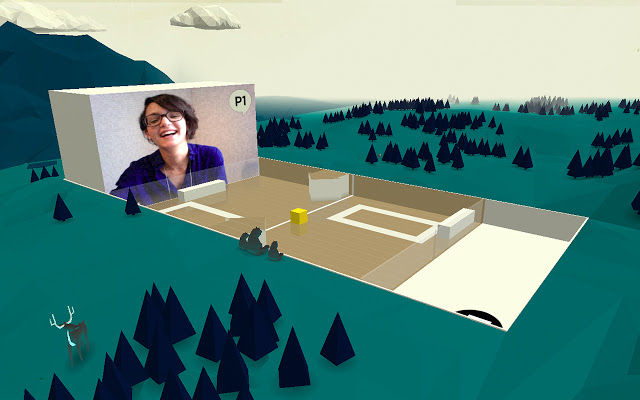
\includegraphics[width=0.70\textwidth]{bilder/cubeslam.jpg}
\caption{Google CubeSlam, mit integriertem WebRTC Videostream.}
\source{\url{https://experiments.withgoogle.com/cube-slam}}
\label{fig:cuubslam}
\end{figure}

Im Bereich der Rundenbasierten Brettspieleentwicklung im Browser findet WebRTC hingegen nur begrenzt Anwendung. Diese beschränkt sich primär auf die zuvor beschriebene Nutzung für Audio- und Videokommunikation.\par
